\documentclass{beamer}
%[aspectratio=169]   \usepackage[czech]{babel}
\usepackage{apo-lecture}
\usepackage{pdfpages}
\usepackage{pdfcomment}
\usepackage{listings}

\subtitle{Lekce 11. Architektura x86}
\author{Petr Štěpán\\ \small\texttt{stepan@fel.cvut.cz}}
\begin{document}

\maketitle

\section{Historie x86}

\begin{frame}
\frametitle{Procesor -- CPU}
\begin{columns}[t,onlytextwidth]
\begin{column}{0.4\textwidth}
Základní vlastnosti:
  \begin{itemize}
    \item šířka datové a adresové sběrnice
    \item počet a velikost vnitřních registrů
    \item rychlost řídicího signálu – frekvence
    \item instrukční sada
  \end{itemize}
\end{column}
\begin{column}{0.52\textwidth}  
   \begin{center}
   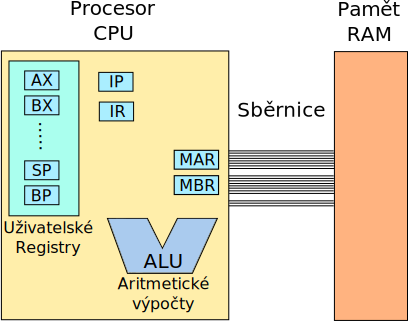
\includegraphics[width=0.9\textwidth]{cpu-cz.pdf}
   \end{center}
\end{column}
\end{columns}
\end{frame}


\begin{frame}
\frametitle{Historie -- x86/AMD64}
\begin{itemize}
\item x86 - rodina procesorů, x je zkratka pro hodnoty x - 0,1,2,3,4,5,6
\end{itemize}

\begin{columns}[t,onlytextwidth]
\begin{column}{0.48\textwidth}
\textbf{8086} -- R16 A20 (1978) první IBM PC (8088 - 1979) \\
\textbf{80286} -- R16 A24 (1982) protected mode\\
\textbf{80386} -- R32 A32 (1985) stránkování\\
\textbf{80486} -- R32 A32 (1989) pipelining, FPU, cache\\
\textbf{80586} -- R32 A32 (1993) Pentium superscalar\\
\end{column}
\begin{column}{0.48\textwidth}  
\textbf{80686} -- R32 A36 (1995) Pentium Pro PAE, L2 cache, out-of-order \& speculative exec\\
\textbf{IA-64} -- R64 A52 (2001) Itanium 64-bitová verze\\
\textbf{AMD64} -- R64 A40 (2003) Athlonn 64-bitová verze od AMD\\
\textbf{Core2} -- R64 A36 (2006) Intel 64 EM64T, SSSE3, $\mu$op, virtualization
\end{column}
\end{columns}

\begin{itemize}
\item Přehledný popis -- \url{https://en.wikibooks.org/wiki/X86\_Assembly}
\end{itemize}

\end{frame}

\begin{frame}[shrink=1.2]
\frametitle{Registry -- x86/AMD64}
\small
Uživatelské registry
\begin{itemize}
\item Všechny registry vzhledem ke zpětné kompatibilitě jsou 64/32/16/8 bitové
\item obecné registry pro ukládání hodnot programu \texttt{eax}, \texttt{ebx}, \texttt{ecx}, \texttt{edx}
\item registry specializované jako ukazatel do paměti \texttt{esi}, \texttt{edi}, \texttt{ebp}
\item \texttt{esp} – stack pointer -- ukazatel zásobníku - detailněji dále
\item AMD64/EM64T přidává 8 dalších registrů \texttt{r8}-\texttt{r15},ve formě \texttt{r8b} nejnižší bajt, \texttt{r8w} nejnižší slovo (16 bitů), \texttt{r8d} – nižších 32 bitů, \texttt{r8} – 64 bitový registr
\end{itemize}
\begin{center}
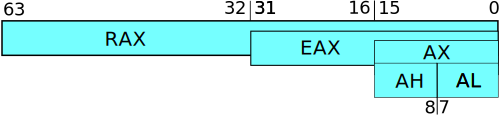
\includegraphics[width=0.5\textwidth]{registers.pdf}
\end{center}
Řídicí a stavové registry
\begin{itemize}
\item \texttt{IP/EIP/RIP} – instruction pointer – adresa zpracovávané instrukce
\item \texttt{FLAGS/EFLAGS/RFLAGS} – stav procesoru
\end{itemize}

\end{frame}



\begin{frame}
\frametitle{Registr FLAGS}
RFLAGS registr
\begin{center}
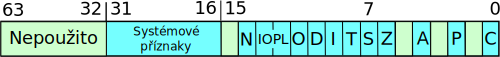
\includegraphics[width=0.65\textwidth]{flags-cz.pdf}
\end{center}
\begin{columns}[t,onlytextwidth]
\begin{column}{0.5\textwidth}
C -- Carry flag\\
P -- Parity flag\\
Z -- Zero flag\\
S -- Sign flag\\
O -- Overflow flag\\
A -- Auxiliary flag (BCD)
\end{column}
\begin{column}{0.5\textwidth}  
I -- Interrupt enable\\
T -- Trap flag\\
IOPL -- I/O privilege level\\
Systémové příznaky:
\begin{itemize}
\item VM -- Virtual 8086 Mode
\item VIF -- Virtual Interrupt Flag
\item VIP -- Virtual Interrupt Pending
\end{itemize}
\end{column}
\end{columns}
\end{frame}

\begin{frame}
\frametitle{Režimy práce procesoru}
FLAGS registr 
\begin{itemize}
  \item Dva režimy práce procesoru IOPL -- základ hardwarových ochran
  \begin{itemize}
    \item CPL0\footnote{Current privilege level} = privilegovaný (systémový) režim
    \begin{itemize}
      \item procesor může vše, čeho je schopen
    \end{itemize}
    \item CPL3 = uživatelský (aplikační) režim
    \begin{itemize}
      \item privilegované operace  jsou zakázány
    \end{itemize}
  \end{itemize}
  \item Privilegované operace
  \begin{itemize}
    \item ovlivnění stavu celého systému (halt, reset, Interrupt Enable/Disable, modifikace Flags,  modifikace registrů MMU ) 
    \item instrukce pro vstup/výstup (in, out)
  \end{itemize}

  \item Přechody mezi režimy
  \begin{itemize}
    \item Po zapnutí stroje systémový režim
    \item Přechod do uživatelského – modifikace Flags (popf nebo reti)
    \item Přechod do systémového – pouze přerušení vč. programového
  \end{itemize}
\end{itemize}
\end{frame}


\section{Instrukce x86}

\begin{frame}
\frametitle{Instrukce – x86/AMD64}
Instrukce ``ulož hodnotu''\\
(běžně se používají dvě různé syntaxe pro zápis assembleru)\\

\begin{tabular}{ l l }
\textbf{AT\&T} & \textbf{Intel}\\
\texttt{movq} zdroj 64b, cíl &	\texttt{mov} cíl, zdroj\\
\texttt{movl} zdroj 32b, cíl &\\
\texttt{movw} zdroj 16b, cíl &\\
\texttt{movb} zdroj 8b, cíl &\\
registry se značí &\\
\texttt{\%ax}	& pouze \texttt{ax}\\
hodnoty \$, hex 0x & číslo, hex postfix h\\
&\\
\texttt{movl \$0xff, \%ebx} & \texttt{mov ebx, 0ffh}\\
\end{tabular}

Pokud je zdroj menší než cíl, existují dvě verze:
\begin{itemize}
 \item movsX -- sign extension, na nejvyšší bity zopakuj znaménko
 \item movzX -- zero extension, nejvyšší bity vynuluj
\end{itemize}
 
\end{frame}


\begin{frame}
\frametitle{Instrukce – x86/AMD64}
Načti hodnotu z adresy (odkaz do paměti)\\
\begin{tabular}{ l l}
AT\&T & Intel \\
\texttt{movl (\%ecx),\%eax} & \texttt{mov eax, [ecx]}\\
\texttt{movl 3(\%ebx), \%eax} & \texttt{mov eax, [ebx+3]} \\
\texttt{movl (\%ebx, \%ecx, 0x2), \%eax} & \texttt{mov eax, [ebx+ecx*2h]} \\
\texttt{movl -0x20(\%ebx, \%ecx, 0x4), \%eax} & \texttt{mov eax, [ebx+ecx*4h-20h]} \\
\end{tabular}

\begin{itemize}
\item odkaz má 4 složky: \emph{základ+index*měřítko+posun}
\item \emph{měřítko} může nabývat hodnot 1,2,4,8
\item lze implementovat přístup do pole struktur: \emph{základ} je ukazatel na první prvek, \emph{index*měřítko} říká, který prvek chceme a \emph{posun}, kterou položku uvnitř struktury potřebujeme.
\item není potřeba použít všechny 4 složky 
\end{itemize}
\end{frame}


\begin{frame}
\frametitle{Instrukce opakování – x86/AMD64}
Instrukce pro řetězce  - \texttt{REP} opakování pro pole hodnot
\begin{itemize}
\item opakuj dokud \texttt{ecx>0}:
\begin{itemize}
\item \texttt{operace (\%esi), (\%edi)}
\item \texttt{esi += d*operand\_size}
\item \texttt{edi += d*operand\_size}
\item \texttt{ecx - -}
\end{itemize}
\item operace může být \texttt{movs, cmps, lods, stos, scas, ins, outs}
\item \texttt{d} - určuje směr a je buď +1, nebo -1
\item \texttt{REP} opakování podle hodnoty \texttt{ecx}
\item \texttt{REPE/REPNE} opakování podle hodnoty \texttt{ecx} a podle porovnání
  \begin{itemize}
  \item operace \texttt{cmps} se navíc zastaví, pokud je/není rozdíl mezi \texttt{(edi)} a \texttt{(esi)} 
  \item operace \texttt{scas} se navíc zastaví, pokud je/není rozdíl mezi \texttt{(edi)} a hodnotou v registru \texttt{eax} 
  \end{itemize}
\end{itemize}

\end{frame}


\begin{frame}[fragile]
\frametitle{Instrukce opakování – x86/AMD64}
Příklad nastav pole na hodnotu -1:
\begin{minted}[fontsize=\footnotesize]{c}
int array[128];
for (int i=0; i<128; i++) {
  array[i]=-1;
}
\end{minted}
přeloženo:
\begin{minted}[fontsize=\footnotesize]{gas}
mov   array, %edi  ; Nastav do edi ukazatel na začátek pole
mov   $128,  %ecx  ; Nastav počet opakování
mov   $-1,   %eax  ; Nastav hodnotu pro uložení
rep   stosd        ; Vyplň celé pole
\end{minted}
\end{frame}

\begin{frame}[fragile]
\frametitle{Instrukce opakování – x86/AMD64}

Najdi konec řetězce:
\begin{minted}[fontsize=\footnotesize]{c}
char str[128];
int i;
for (i=0; i<128; i++) {
  if (str[i]==0) 
    break;
}
\end{minted}
přeloženo:
\begin{minted}[fontsize=\footnotesize]{gas}
mov   str,  %edi  ; Nastav do EDI začátek pole
mov   $128, %ecx  ; Nastav počet opakování
mov   $0,   %eax  ; Nastav hodnotu konce řetězce
repne scasb       ; Projdi str a najdi hodnotu 0
\end{minted}

\end{frame}



\begin{frame}
\frametitle{Instrukce – x86/AMD64}
Aritmetika -- AT\&T syntax

následující instrukce mají argumenty typu X -- b, w, l, q
\begin{tabular}{ l l}
operace co, k čemu &\\
\texttt{addq    \$0x05,\%rax} & rax = rax + 5\\
\texttt{subl    -4(\%ebp), \%eax} &  eax = eax -- mem(ebp-4)\\
\texttt{subl    \%eax, -4(\%ebp)} & mem(ebp-4) = mem(ebp-4)-eax\\
\texttt{andX} co , k čemu& bitový and\\
\texttt{orX} co , k čemu& bitový or\\
\texttt{xorX} co , k čemu& bitový xor (nejrychlejší vynulování registru)\\
\texttt{mulX} čím & násobení eax číslem bez znamének\\
\texttt{divX} čím & dělení edx:eax číslem bez znamének\\
\texttt{imulX} čím & násobení eax číslem se znaménky\\
\texttt{idivX} čím & dělení edx:eax číslem se znaménky\\
\end{tabular}
\end{frame}

\begin{frame}
\frametitle{Instrukce – x86/AMD64}
Aritmetika s jedním operandem -- AT\&T syntax
\begin{tabular}{ l l}
operace   s cim&\\
\texttt{incl            \%eax} &              eax = eax + 1\\
\texttt{decw            (\%ebx)} &                 mem(ebx) = mem(ebx)-1\\
\texttt{shlb            \$3, \%al} &                al = al$<<$3\\
\texttt{shrb            \$1, \%bl} &                bl=11000000, po bl=01100000\\
\texttt{sarb            \$1, \%bl} &                bl=11000000, po bl=11100000\\
\texttt{rorX, rolX} & bitová rotace doprava a doleva\\
\texttt{rcrX, rclX} & bitova rotace přes C -- carry flag\\
\end{tabular}
\end{frame}


\begin{frame}
\frametitle{Instrukce – x86/AMD64}
Podmíněné skoky\\
\begin{tabular}{ l l}
\texttt{test    a1, a2} &  tmp = a1 AND a2, Z tmp=0, C tmp<0\\
\texttt{cmp     a1, a2} &  tmp = a1-a2, Z tmp=0, C tmp<0\\
\end{tabular}

pak lze použít následující skoky
\begin{tabular}{ l l}
\texttt{jmp kam} & nepodmíněný skok, vlastně \texttt{\%eip=kam}\\
\texttt{je      kam} & jmp equal -- skoč při rovnosti\\
\texttt{jne kam} & jmp not equal -- skoč při nerovnosti\\
\texttt{jg/ja kam} & jmp greater – skoč pokud je a1 > a2 (sign/unsig)\\
\texttt{jge/jae kam} & skoč pokud je a1 >= a2 (sign/unsig)\\
\texttt{jl/jb kam} & jmp less – skoč pokud je a1 < a2 (sign/unsig)\\
\texttt{jle/jbe kam} & skoč pokud je a1 <= a2 (sign/unsig)\\
\texttt{jz/jnz kam} & skoč pokud je Z=1/0\\
\texttt{jo/jno kam}& skoč pokud je O (overflow) = 1/0\\
\end{tabular}
\end{frame}

\begin{frame}
\frametitle{Quiz}
Liší se velikost programů pro CISC (x86) a RISC (RISC V)?
\begin{itemize}
\item[A] neliší, je přibližně stejná
\item[B] programy pro CISC jsou delší
\item[C] programy pro RISC jsou delší
\end{itemize}

\end{frame}


\begin{frame}[fragile]
\frametitle{Porovnání CISC vs. RISC}
CISC programy jsou většinou kratší:
\begin{minted}[fontsize=\footnotesize]{gas}
incl 10(%ecx)   -      lw   t2, 10(t1)
                       addi t2, t2, 1
                       sw   t2, 10(t1)

rep movs        - l1:  lw   t3, 0(t1) 
                       sw   t3, 0(t2)
                       addi t1, t1, 4
                       addi t2, t2, 4
                       addi t4, t4, -1
                       jne  t4, zero, l1 
\end{minted}

\end{frame}

\begin{frame}
\frametitle{Quiz}
Jsou programy pro CISC (x86) rychlejší než pro RISC (RISC V)?
\begin{itemize}
\item[A] Ano 
\item[B] Ne
\item[C] Jak kdy, záleží na procesoru
\end{itemize}

\end{frame}



\begin{frame}
\frametitle{Zásobník}

\begin{columns}
\begin{column}{0.45\textwidth}
\small
Zásobník:
\begin{itemize}
\item datová struktura LIFO
\end{itemize}

Implemetace:
\begin{itemize}
\item implementace registrem \textit{SP} - ukazuje na vrchol zásobníku
\item konvence - při každém pop se zvětšuje registr \textit{SP} o velikost operandu, při push se \textit{SP} zmenšuje.
\end{itemize}
\begin{tabular}{ l l}
\texttt{pushl \%eax} &  ulož eax na zásobník\\
\texttt{popw \%bx}   &  vyber ze zásobníku \\
                     &  2 bajty do \textit{bx}\\
\texttt{pushf/popf}  &  ulož/vyber register\\
                     &  EFLAGS\\
\texttt{pusha/popa}  &  ulož/vyber všechny\\
                     &  uživatelské registry\\
\end{tabular}
\end{column}

\begin{column}{0.55\textwidth}  
\small
\begin{itemize}
\item operace push vloží data do zásobníku
\begin{itemize}
\item \texttt{sub \$size, sp}
\item \texttt{mov \%eax, 0(sp)}
\end{itemize}
\item operace pop vybere data ze zásobníku
\begin{itemize}
\item \texttt{mov 0(sp), \%eax}
\item \texttt{add \$size, sp}
\end{itemize}
\item lze k zásobníku přistupovat podobně, jako v RISC-V:
\begin{itemize}
\item \texttt{sub \$16, sp}
\item \texttt{mov \%eax, 0(sp)}
\item \texttt{mov \%ebx, 4(sp)}
\item \texttt{mov \%ecx, 8(sp)}
\item \texttt{mov \%edx, 12(sp)}
\end{itemize}
\end{itemize}
\end{column}
\end{columns}
\end{frame}


\begin{frame}[fragile]
\frametitle{Kvíz}

Který program provede superskalární architektura rychleji:
\begin{columns}
\begin{column}{0.45\textwidth}
A
\begin{minted}[fontsize=\footnotesize]{gas}
push %eax
push %ebx
push %ecx
push %edx
\end{minted}
\end{column}
\hfill
\begin{column}{0.45\textwidth}  
B
\begin{minted}[fontsize=\footnotesize]{gas}
sub $16, sp
mov %eax, 0(sp)
mov %ebx, 4(sp)
mov %ecx, 8(sp)
mov %edx, 12(sp)
\end{minted}
\end{column}
\end{columns}

\begin{itemize}
\item[A] Oba přibližně stejně
\item[B] A rychleji než B
\item[C] B rychleji než A
\item[D] Nelze určit
\end{itemize}
\end{frame}

\begin{frame}
\frametitle{Volání funkce -- x86 cdecl}

\begin{itemize}
\item Volající uloží na zásobník všechny parametry
\item Pořadí ukládání na zásobník je od posledního parametru k prvnímu
\end{itemize}

\bigskip

Volání funkce\\
\begin{tabular}{ l l}
\texttt{call adr} &         vlastně \texttt{push \%eip}, \texttt{jmp adr}\\
\end{tabular}\\
Návrat z funkce\\
\begin{tabular}{ l l}
\texttt{ret} &              vlastně \texttt{pop \%eip}\\
\end{tabular}\\
\bigskip

\begin{itemize}
\item Návratová hodnota funkce bude uložena v registru eax.
\item Registry ebp, ebx, esi, edi nesmí funkce změnit. Pokud je chce funkce využít, musí být uložena původní hodnota na zásobník.
\end{itemize}

\end{frame}


\begin{frame}[fragile]
\frametitle{Volání funkce -- x86 -- rámec funkce}
Registr ebp ukazuje na zásobník, kam byla uložena stará hodnota rámce předchozí funkce\\
\bigskip
Úvod funkce – příklad implementace
\begin{minted}[fontsize=\footnotesize]{gas}
push  %ebp        ; Uložíme hodnotu EBP do zasobníku
mov   %esp, %ebp  ; Nastav EBP na současnou hodnotu zasobníku
sub   $12, %esp   ; Připrav místo na zasobníku pro 12 bajtů
                  ; lokálních proměnných
\end{minted}

První proměnná bude na adrese \texttt{-4(\%ebp)}, druha \texttt{-8(\%ebp)}\\
První parametr bude na adrese \texttt{8(\%ebp)}, další \texttt{12(\%ebp)}

Ukončení funkce:
\begin{minted}[fontsize=\footnotesize]{gas}
mov   %ebp, %esp  ; Vrať stav zásobníku na původní pozici.
pop   %ebp        ; Obnov puvodní hodnotu registru EBP
ret               ; Návrat z funkce
\end{minted}

Speciální instrukce pro návrat z funkce:
\texttt{leave} vlastně: 
\begin{minted}[fontsize=\footnotesize]{gas}
mov   %ebp, %esp 
pop   %ebp        
\end{minted}

\end{frame}

\begin{frame}[fragile]
\frametitle{Volání funkce -- x86 -- příklad}

\begin{columns}
\begin{column}{0.35\textwidth}
Volání funkce:

\begin{minted}[fontsize=\footnotesize]{c}
t = secti(1, 2, 3, 4);
\end{minted}

Překlad do x86
\begin{minted}[fontsize=\footnotesize]{gas}
push $4
push $3
push $2
push $1
call 10e2 <secti>
add $0x10, %esp
\end{minted}
\end{column}


\begin{column}{0.35\textwidth}  
Začátek funkce
\begin{minted}[fontsize=\footnotesize]{gas}
push %ebp
mov  %esp, %ebp
push %ebx
sub  $0x10, %esp
\end{minted}

Lokální proměnné
\begin{minted}[fontsize=\footnotesize]{gas}
mov %eax, -4(ebp)
\end{minted}

První a druhý parametr:
\begin{minted}[fontsize=\footnotesize]{gas}
mov 0x8(ebp), %edx
mov 0xc(ebp), %eax
\end{minted}

Zakončení funkce:
\begin{minted}[fontsize=\footnotesize]{gas}
leave
ret
\end{minted}
\end{column}

\begin{column}{0.3\textwidth}  
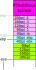
\includegraphics[width=0.95\textwidth]{fnc_frame-cz.pdf}
\end{column}

\end{columns}
\end{frame}


\begin{frame}
\frametitle{Volání funkce -- AMD64 Linux}

\begin{itemize}
\item Volající uloží do registrů rdi, rsi, rdx, rcx, r8, r9, zmm0-7 prvních 6 parametrů celočíselných, nebo 8 parametrů reálných čísel
\item Ostatní parametry na zásobník
\end{itemize}

\bigskip

\begin{itemize}
\item Návratová hodnota funkce bude uložena v registru rax a rdx.
\item Registry rbp, rbx, r12-r15 nesmí funkce změnit. Pokud je chce funkce využít musí být uložena původní hodnota na zásobník.
\item Red Zone -- zóna 128 bajtů od pointeru rsp, kterou nesmí měnit obsluha přerušení. Tato zóna umožňuje využívat tuto paměť pro dočasné proměnné bez posunování rsp ukazatele.
Samozřejmě volání funkce tuto zónu mění.
\end{itemize}

\end{frame}



\begin{frame}
\frametitle{Funkce zásobníku}

Zásobník:
\begin{itemize}
  \item parametry pro funkci
  \item kam se vrátit po ukončení funkce, místo odkud program volal funkci
  \item lokální proměnné funkce
  \begin{itemize}
    \item zásobník je vetšinou malý
    \item omezená velikost lokálních proměnných
    \item pozor při rekurzi - lépe se rekurzi vyhnout
  \end{itemize}
\end{itemize}

\end{frame}



\begin{frame}[fragile]
\frametitle{Quiz}

Mějme program:
\begin{columns}
\begin{column}{0.45\textwidth}
\begin{lstlisting}[language={C},columns=flexible]
int factorial(int x) {
  int y;
  if (x<=1) {
    return 1;
  } else {
    y = factorial(x-1)
    return y*x;
  }
}
\end{lstlisting}
\end{column}
\hfill
\begin{column}{0.45\textwidth}  
\begin{lstlisting}[language={C},columns=flexible]
int i;
int main() {
  i=10;
  i=factorial(i);
  return i;
}
\end{lstlisting}
\end{column}
\end{columns}

Kde se bude nacházet proměnná i?
\begin{itemize}
\item[A] Pro RISC V i pro x86 na zásobníku.
\item[B] Pro RISC V dynamicky alokovaná, pro x86 na zásobníku.
\item[C] Pro RISC V i pro x86 na místě v paměti určeném při překladu.
\item[D] Pro RISC V i pro x86 pouze v registru.
\end{itemize}
\end{frame}


\begin{frame}[fragile]
\frametitle{Quiz}

Mějme program:
\begin{columns}
\begin{column}{0.45\textwidth}
\begin{lstlisting}[language={C},columns=flexible]
int factorial(int x) {
  int y;
  if (x<=1) {
    return 1;
  } else {
    y = factorial(x-1)
    return y*x;
  }
}
\end{lstlisting}
\end{column}
\hfill
\begin{column}{0.45\textwidth}  
\begin{lstlisting}[language={C},columns=flexible]
int i;
int main() {
  i=10;
  i=factorial(i);
  return i;
}
\end{lstlisting}
\end{column}
\end{columns}

Kde se bude nacházet proměnná y při překladu bez optimalizace?
\begin{itemize}
\item[A] Pro RISC V i pro x86 na zásobníku nebo v registru
\item[B] Pro RISC V i pro x86 dynamicky alokovaná
\item[C] Pro RISC V i pro x86 na místě v paměti určeném při překladu
\item[D] Pro RISC V i pro x86 nelze určit
\end{itemize}
\end{frame}

\begin{frame}[fragile,shrink=10]
\frametitle{Quiz}

Mějme program:
\begin{columns}
\begin{column}{0.45\textwidth}
\begin{lstlisting}[language={C},columns=flexible]
int factorial(int x) {
  int y;
  if (x<=1) {
    return 1;
  } else {
    y = factorial(x-1)
    return y*x;
  }
}
\end{lstlisting}
\end{column}
\hfill
\begin{column}{0.45\textwidth}  
\begin{lstlisting}[language={C},columns=flexible]
int i;
int main() {
  i=10;
  i=factorial(i);
  return i;
}
\end{lstlisting}
\end{column}
\end{columns}

Kde se bude nacházet proměnná x při překladu bez optimalizace?
\begin{itemize}
\item[A] Pro RISC V i pro x86 na zásobníku
\item[B] Pro RISC V v registru, pro x86 na zásobníku
\item[C] Pro RISC V v registru a následně bude uložena na zásobník, pro x86 na zásobníku
\item[D] Pro RISC V na zásobníku, pro x86 v registru
\item[E] Pro RISC V na zásobníku, pro x86 v registru a následně na zásobníku
\end{itemize}
\end{frame}

\begin{frame}[fragile,shrink=10]
\frametitle{Quiz}

Mějme program:
\begin{columns}
\begin{column}{0.45\textwidth}
\begin{lstlisting}[language={C},columns=flexible]
int factorial(int x) {
  int y;
  if (x<=1) {
    return 1;
  } else {
    y = factorial(x-1)
    return y*x;
  }
}
\end{lstlisting}
\end{column}
\hfill
\begin{column}{0.45\textwidth}  
\begin{lstlisting}[language={C},columns=flexible]
int i;
int main() {
  i=10;
  i=factorial(i);
  return i;
}
\end{lstlisting}
\end{column}
\end{columns}

Kde se bude nacházet návratová adresa z funkce factorial?
\begin{itemize}
\item[A] Pro RISC V i pro x86 na zásobníku
\item[B] Pro RISC V v registru, pro x86 na zásobníku
\item[C] Pro RISC V v registru a následně bude uložena na zásobník, pro x86 na zásobníku
\item[D] Pro RISC V na zásobníku, pro x86 v registru
\item[E] Pro RISC V na zásobníku, pro x86 v registru a následně na zásobníku
\end{itemize}
\end{frame}



\begin{frame}
\frametitle{Instrukce – x86/AMD64}
Složitost assembleru
\begin{itemize}
\item Algoritmus se dá přeložit různými způsoby do assembleru
\item Strojový překlad je někdy hodně kostrbatý
\begin{itemize}
\item např. \texttt{mov 0x12345, \%esi; mov \%esi, \%ebx} místo \texttt{mov 0x12345, \%ebx}
\end{itemize}
\item Různé způsoby pracují různě rychle a jsou rozdílně dlouhé a rozdílně přehledné
\begin{itemize}
\item \texttt{xor \%ebx, \%ebx}  je to samé jako \texttt{ mov \$0, \%ebx}
\item \texttt{lea} adresa, registr – load effective address – nastaví hodnotu ukazatele do zadaného registru
\item \texttt{lea   -12(\%esp), \%esp }  je to samé jako \texttt{ sub    \$12, \%esp} 
\item lea je výhodnější vzhledem k předzpracování instrukcí, nezatěžuje ALU jednotku (ovšem třeba Atom má zpracování adr. pomalejší než ALU).
\end{itemize}
\end{itemize}
\end{frame}

\section{FPU - x87}


\begin{frame}
\frametitle{FPU coprocesor – x87}
Speciální součást procesoru pro práci s reálnými čísly
\begin{itemize}
\item Podporuje single-32, double-64, extended-80 i exotické formáty BCD
\item Obsahuje vlastních 8 registrů o 80 bitech
\item Registry jsou organizovány v zásobníku (push, pop), ale umožňují i přímý přístup (0-7)
\item Každá operace pracuje s vrcholem zásobníku a jedním dalším registrem, nebo hodnotou
\item Původně oddělený procesor, od 486 on-die -- na jednom čipu
\item Podporuje všechny IEEE-754 operace:
\begin{itemize}
\item fadd, fsub, fmul, fdiv, fsqrt, fcmp, fsin, ...
\end{itemize}
\end{itemize}
\end{frame}

\begin{frame}
\frametitle{Způsob práce FPU}
Základní operace slouží pro uložení reálného čísla z/do registrů:
\begin{itemize}
\item fld - uloží hodnotu z paměti na zásobník registrů -- push
\item fst - uloží hodnotu z registru do paměti bez pop
\item fstp - uloží hodnotu z registru do paměti a udělá pop
\end{itemize}
Základní operace pro uložení celého čísla (integer) z/do registrů:
\begin{itemize}
\item fild - uloží celé číslo z paměti na zásobník registrů -- push
\item fist - uloží celé číslo z registru do paměti bez pop
\item fistp - uloží celé číslo z registru do paměti a udělá pop
\item fisttp - uloží zaokrouhlené celé číslo z registru do paměti a udělá pop
\end{itemize}
\end{frame}

\begin{frame}
\frametitle{Operace FPU}
Práci základních operací si ukážeme na sčítání (ostatní operace mají shodný tvar, ST(0) je vrchol zásobníku, ST(1) hodnota pod ním, atd.):
\begin{itemize}
\item fadd float/double - přičti obsah paměti k ST(0) a výsledek ulož do ST(0)
\item fiadd short/int - přičti celé číslo z paměti k ST(0) a výsledek ulož do ST(0)
\item fadd ST(0), ST(i) - sečti obsah ST(0) a ST(i) a výsledek ulož do ST(0)
\item fadd ST(i), ST(0) - sečti obsah ST(i) a ST(0) a výsledek ulož do ST(i)
\item faddp ST(i), ST(0) - sečti obsah ST(i) a ST(0) a výsledek ulož do ST(i) a udělej pop operaci (zruš hodnotu ST(0))
\item faddp - sečti obsah ST(1) a ST(0) a výsledek ulož do ST(1) a udělej pop operaci (zruš hodnotu ST(0))
\end{itemize}
\end{frame}


\begin{frame}
\frametitle{Operace FPU}
Operace SUB a DIV mají navíc i reverzní formu, tedy otočení pořadí operandů (ve všech verzích, jak s pamětí, tak s registry):
\begin{itemize}
\item fsub ST(0), ST(i) - výsledek ST(0) - ST(i) ulož do ST(0)
\item fsubr ST(0), ST(i) - výsledek ST(i) - ST(0) ulož do ST(0)
\end{itemize}

Unární funkce sin, cos:
\begin{itemize}
\item fsin/fcos - ST(0) nahraď hodnotou sin/cos(ST(0))
\end{itemize}

Logaritmus - výpočet $y\cdot\log_2 x$:
\begin{itemize}
\item fyl2x - ST(1) nahraď hodnotou ST(1)*($log_2$ ST(0)) a udělej pop
\end{itemize}

Načtení konstant:
\begin{itemize}
\item fldz/fld1 - uloží 0.0/1.0 na zásobník 
\item fldpi/fldl2e - uloží $\pi$/$\log_2 e$ na zásobník 
\end{itemize}

\end{frame}


\begin{frame}[fragile]
\frametitle{Příklad programu s FPU}
Příklad výpočtu 1.1*2.2+sin(3.3):
\begin{lstlisting}[language={[x86masm]Assembler},columns=flexible]
fldl   adr_1.1  ; Nacteme prvni operand
fmull  adr_2.2  ; Vynasobime prvni op druhym op
fldl   adr_3.3  ; Nacteme treti operand
fsinl           ; Spocti sin tretiho operandu
faddp           ; Secti dve cisla a ponech jen soucet
fstp   adr_vysl ; Uloz vysledek do pameti
\end{lstlisting}

\end{frame}


\begin{frame}
\frametitle{FPU pro RISC V}
\begin{itemize}
\item Dvě rozšíření RV64F – float, RV64D – double
\item 32 interních registrů, buď o velikosti 32 bitů pro float, nebo o velikosti 64 bitů pro double
\item Nové instrukce pro načtení load a store – flw, fsw (fld, fsd)
\item Nové instrukce pro operace:
\begin{itemize}
\item fadd.s, fsub.s, fmul.s, fdiv.s ( *.d pro double)
\item fadd.s   F[rd]=F[rs1]+F[rs2] 
\item fsqrt.s -- square root -- odmocnina  F[rd] = sqrt(F[rs1])
\item fmadd.s -- násob a sečti, F[rd]=F[rs1]*F[rs2]+F[rs3]
\item fmsub.s -- násob a odečti, F[rd]=F[rs1]*F[rs2]-F[rs3]
\item fmin.s -- F[rd] = (F[rs1]<F[rs2]) ? F[rs1] : F[rs2]
\item převody mezi float, double a celými čísly
\end{itemize}
\end{itemize}
\end{frame}

\section{Rozšíření MMX}


\begin{frame}
\frametitle{SIMD - MMX}

\begin{itemize}
\item SIMD - Single Instruction Multiple Data - provedení jednoho typu instrukce na více datech najednou
\item MMX - MultiMedia eXtension (někdy se vysvětluje jako Multiple Math eXtension)
\item Využívají stejné registry jako FPU x87, nelze je tedy používat současně
\item 64-bitový registr může fungovat v následujících módech:
\begin{itemize}
\item B - $8\times$ bajt
\item W - $4\times$ short int
\item D - $2\times$ int
\end{itemize}
\item Operace: 
\begin{itemize}
\item Aritmetické - sčítání, odčítání, násobení
\item Logické - and, or, rotace, porovnání
\item Konverze - pack, přesuny mezi registry
\end{itemize}
\end{itemize}
\end{frame}

\begin{frame}
\frametitle{MMX operace}
\begin{columns}[t,onlytextwidth]
  \begin{column}{0.5\textwidth}
    \texttt{PADDW} - součet po částech (packed)
  \end{column}
  \begin{column}{0.5\textwidth}
    \texttt{PADDUSW} - součet saturovaný (bez přetečení)
  \end{column}
\end{columns}
\begin{columns}[t,onlytextwidth]
  \begin{column}{0.5\textwidth}
    \begin{center}
    
\includegraphics[width=0.8\textwidth]{mmx-add.pdf}
    \end{center}
  \end{column}
  \begin{column}{0.5\textwidth}
    \begin{center}
    
\includegraphics[width=0.8\textwidth]{mmx-add-sat.pdf}
    \end{center}
  \end{column}
\end{columns}

\end{frame}

\begin{frame}
\frametitle{MMX operace}
\small
    \begin{center}
    \texttt{PMADDWD} - vynásob a sečti\\
    
\includegraphics[width=0.4\textwidth]{mmx-mul-add.pdf}
    \end{center}
\vspace{-1cm}
\begin{columns}[t,onlytextwidth]
  \begin{column}{0.5\textwidth}
    \begin{center}
    \texttt{PMULLW} - součin (spodní část)
    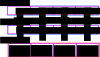
\includegraphics[width=0.8\textwidth]{mmx-mull.pdf}
    \end{center}
  \end{column}
  \begin{column}{0.5\textwidth}
    \begin{center}
    \texttt{PMULHW} - součin (vrchní část)
    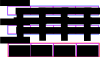
\includegraphics[width=0.8\textwidth]{mmx-mulh.pdf}
    \end{center}
  \end{column}
\end{columns}


\end{frame}


\begin{frame}[fragile]
\frametitle{MMX příklad}

\begin{columns}[t,onlytextwidth]
  \begin{column}{0.5\textwidth}
Maskování obrazu v obraze:
\begin{lstlisting}[language={C},columns=flexible]
unsigned char mask[size],
 obr1[size], obr2[size];
if (mask[i]==0) {
  new_img[i] = obr1[i];
} else {
  new_img[i] = obr2[i];
}
\end{lstlisting}

  \end{column}
  \begin{column}{0.5\textwidth}
MMX implementace 8 pixelů najednou
\begin{lstlisting}[language={[x86masm]Assembler},columns=flexible]
movq    mask_ptr, %mm0
pcmpeqb %mm0, 0
movq    %mm0, %mm1
pand    %mm1, obr1_ptr
pandn   %mm0, obr2_ptr
por     %mm0, %mm1
movq    %mm0, new_img_ptr
\end{lstlisting}
  \end{column}
\end{columns}
\end{frame}




\begin{frame}
\frametitle{3Dnow! rozšíření MMX}
\begin{itemize}
\item Rozšíření 3Dnow! přidalo ve stávajících registrech \texttt{mm0}-\texttt{mm7} práci s reálnými čísly. 
\item Umožňuje pouze dělení registru na dvě reálná čísla po 32bitech
\item Přidává konverzi celých čísel na reálná čísla a zpět, také pomocí průměrování 8-bitových a 16-bitových celých čísel
\item Sčítání, odčítání, násobení, dělení reálných čísel po složkách
\item Porovnávání reálných čísel a nalezení minim a maxim
\end{itemize}
\end{frame}

\section{Rozšíření SSE}


\begin{frame}
\frametitle{SSE další SIMD}
\begin{itemize}
\item SSE - Streaming SIMD Extension
\item nové registry xmm0-xmm7
\item každý registr 128-bitů, možné dělení
\item $4\times$ float - 32-bitové reálné číslo
\item $2\times$ double - 64-bitové reálné číslo
\item rozšíření celočíselných operací MMX na 128-bitové registry
\end{itemize}
\end{frame}



\begin{frame}
\frametitle{Instrukce SSE}
\begin{itemize}

\item Operace: packet suffix -ps, scalar suffix -ss 



\item Uložit z/do paměti: mov
\item Aritmetické operace float: add, sub, mul, div, rcp, sqrt, max, min, rsqrt
\item Logické operace: and, or, xor, andn
\item Porovnání: cmp, comi, ucomi


\item Scalar operation: addss, subss, mulss, divss
\end{itemize}
\end{frame}

\begin{frame}
\frametitle{Packet SSE}
\begin{columns}[t,onlytextwidth]
\begin{column}{0.5\textwidth}
\begin{center}
Packet operation

\includegraphics[width=0.9\textwidth]{sse.pdf}
\end{center}
\end{column}
\begin{column}{0.5\textwidth}
\begin{center}
Scalar operation

\includegraphics[width=0.9\textwidth]{sse-s.pdf}
\end{center}
\end{column}
\end{columns}
\end{frame}

\begin{frame}
\frametitle{Rozšíření SSE}
Další rozšíření:
\begin{itemize}
\item SSE2 - přidala dalších 144 nových instrukcí
\item SSE3 - dalších 13 instrukcí
\item SSSE3 - dalších 16 instrukcí
\item SSE4 - dalších 47 nových instrukcí
\item SSE4.2 - dalších 170 nových instrukcí
\end{itemize}
\end{frame}


\end{document}

